\documentclass[]{article}
\usepackage{lmodern}
\usepackage{amssymb,amsmath}
\usepackage{ifxetex,ifluatex}
\usepackage{fixltx2e} % provides \textsubscript
\ifnum 0\ifxetex 1\fi\ifluatex 1\fi=0 % if pdftex
  \usepackage[T1]{fontenc}
  \usepackage[utf8]{inputenc}
\else % if luatex or xelatex
  \ifxetex
    \usepackage{mathspec}
  \else
    \usepackage{fontspec}
  \fi
  \defaultfontfeatures{Ligatures=TeX,Scale=MatchLowercase}
\fi
% use upquote if available, for straight quotes in verbatim environments
\IfFileExists{upquote.sty}{\usepackage{upquote}}{}
% use microtype if available
\IfFileExists{microtype.sty}{%
\usepackage{microtype}
\UseMicrotypeSet[protrusion]{basicmath} % disable protrusion for tt fonts
}{}
\usepackage[margin=1in]{geometry}
\usepackage{hyperref}
\hypersetup{unicode=true,
            pdftitle={Combining perl, c and R},
            pdfauthor={Bruna Wundervald},
            pdfborder={0 0 0},
            breaklinks=true}
\urlstyle{same}  % don't use monospace font for urls
\usepackage{natbib}
\bibliographystyle{apalike}
\usepackage{color}
\usepackage{fancyvrb}
\newcommand{\VerbBar}{|}
\newcommand{\VERB}{\Verb[commandchars=\\\{\}]}
\DefineVerbatimEnvironment{Highlighting}{Verbatim}{commandchars=\\\{\}}
% Add ',fontsize=\small' for more characters per line
\usepackage{framed}
\definecolor{shadecolor}{RGB}{248,248,248}
\newenvironment{Shaded}{\begin{snugshade}}{\end{snugshade}}
\newcommand{\AlertTok}[1]{\textcolor[rgb]{0.94,0.16,0.16}{#1}}
\newcommand{\AnnotationTok}[1]{\textcolor[rgb]{0.56,0.35,0.01}{\textbf{\textit{#1}}}}
\newcommand{\AttributeTok}[1]{\textcolor[rgb]{0.77,0.63,0.00}{#1}}
\newcommand{\BaseNTok}[1]{\textcolor[rgb]{0.00,0.00,0.81}{#1}}
\newcommand{\BuiltInTok}[1]{#1}
\newcommand{\CharTok}[1]{\textcolor[rgb]{0.31,0.60,0.02}{#1}}
\newcommand{\CommentTok}[1]{\textcolor[rgb]{0.56,0.35,0.01}{\textit{#1}}}
\newcommand{\CommentVarTok}[1]{\textcolor[rgb]{0.56,0.35,0.01}{\textbf{\textit{#1}}}}
\newcommand{\ConstantTok}[1]{\textcolor[rgb]{0.00,0.00,0.00}{#1}}
\newcommand{\ControlFlowTok}[1]{\textcolor[rgb]{0.13,0.29,0.53}{\textbf{#1}}}
\newcommand{\DataTypeTok}[1]{\textcolor[rgb]{0.13,0.29,0.53}{#1}}
\newcommand{\DecValTok}[1]{\textcolor[rgb]{0.00,0.00,0.81}{#1}}
\newcommand{\DocumentationTok}[1]{\textcolor[rgb]{0.56,0.35,0.01}{\textbf{\textit{#1}}}}
\newcommand{\ErrorTok}[1]{\textcolor[rgb]{0.64,0.00,0.00}{\textbf{#1}}}
\newcommand{\ExtensionTok}[1]{#1}
\newcommand{\FloatTok}[1]{\textcolor[rgb]{0.00,0.00,0.81}{#1}}
\newcommand{\FunctionTok}[1]{\textcolor[rgb]{0.00,0.00,0.00}{#1}}
\newcommand{\ImportTok}[1]{#1}
\newcommand{\InformationTok}[1]{\textcolor[rgb]{0.56,0.35,0.01}{\textbf{\textit{#1}}}}
\newcommand{\KeywordTok}[1]{\textcolor[rgb]{0.13,0.29,0.53}{\textbf{#1}}}
\newcommand{\NormalTok}[1]{#1}
\newcommand{\OperatorTok}[1]{\textcolor[rgb]{0.81,0.36,0.00}{\textbf{#1}}}
\newcommand{\OtherTok}[1]{\textcolor[rgb]{0.56,0.35,0.01}{#1}}
\newcommand{\PreprocessorTok}[1]{\textcolor[rgb]{0.56,0.35,0.01}{\textit{#1}}}
\newcommand{\RegionMarkerTok}[1]{#1}
\newcommand{\SpecialCharTok}[1]{\textcolor[rgb]{0.00,0.00,0.00}{#1}}
\newcommand{\SpecialStringTok}[1]{\textcolor[rgb]{0.31,0.60,0.02}{#1}}
\newcommand{\StringTok}[1]{\textcolor[rgb]{0.31,0.60,0.02}{#1}}
\newcommand{\VariableTok}[1]{\textcolor[rgb]{0.00,0.00,0.00}{#1}}
\newcommand{\VerbatimStringTok}[1]{\textcolor[rgb]{0.31,0.60,0.02}{#1}}
\newcommand{\WarningTok}[1]{\textcolor[rgb]{0.56,0.35,0.01}{\textbf{\textit{#1}}}}
\usepackage{graphicx,grffile}
\makeatletter
\def\maxwidth{\ifdim\Gin@nat@width>\linewidth\linewidth\else\Gin@nat@width\fi}
\def\maxheight{\ifdim\Gin@nat@height>\textheight\textheight\else\Gin@nat@height\fi}
\makeatother
% Scale images if necessary, so that they will not overflow the page
% margins by default, and it is still possible to overwrite the defaults
% using explicit options in \includegraphics[width, height, ...]{}
\setkeys{Gin}{width=\maxwidth,height=\maxheight,keepaspectratio}
\IfFileExists{parskip.sty}{%
\usepackage{parskip}
}{% else
\setlength{\parindent}{0pt}
\setlength{\parskip}{6pt plus 2pt minus 1pt}
}
\setlength{\emergencystretch}{3em}  % prevent overfull lines
\providecommand{\tightlist}{%
  \setlength{\itemsep}{0pt}\setlength{\parskip}{0pt}}
\setcounter{secnumdepth}{5}
% Redefines (sub)paragraphs to behave more like sections
\ifx\paragraph\undefined\else
\let\oldparagraph\paragraph
\renewcommand{\paragraph}[1]{\oldparagraph{#1}\mbox{}}
\fi
\ifx\subparagraph\undefined\else
\let\oldsubparagraph\subparagraph
\renewcommand{\subparagraph}[1]{\oldsubparagraph{#1}\mbox{}}
\fi

%%% Use protect on footnotes to avoid problems with footnotes in titles
\let\rmarkdownfootnote\footnote%
\def\footnote{\protect\rmarkdownfootnote}

%%% Change title format to be more compact
\usepackage{titling}

% Create subtitle command for use in maketitle
\providecommand{\subtitle}[1]{
  \posttitle{
    \begin{center}\large#1\end{center}
    }
}

\setlength{\droptitle}{-2em}

  \title{Combining \texttt{perl}, \texttt{c} and \texttt{R}}
    \pretitle{\vspace{\droptitle}\centering\huge}
  \posttitle{\par}
    \author{Bruna Wundervald}
    \preauthor{\centering\large\emph}
  \postauthor{\par}
      \predate{\centering\large\emph}
  \postdate{\par}
    \date{May, 2019}

\usepackage{amsmath,amsfonts,amssymb}
\usepackage[ruled,longend]{algorithm2e}
\SetKw{KwBy}{by}
\usepackage{natbib}
\usepackage{float}

\begin{document}
\maketitle

\hypertarget{introduction}{%
\section{Introduction}\label{introduction}}

Music information retrieval is a recent area is a science, which has
been growing fastly. It combines computational tools and music theory to
amplify our knowledge and utility of music data, in the most different
formats. There are many ways of representing music data, such as chords,
lyrics, audio, and so on. Each one of those carries different levels of
information about the songs, and they will be used for distinct tasks.

In \texttt{R}, the \texttt{chorrrds} package is responsible for
extracting music chords of a given artist. The chords come in a
character format, meaning that some treatment needs to be done if we
want to use this data properly. For lyrics data, the \texttt{vagalumeR}
package provides access to the Vagalume API
(\url{https://www.vagalume.com.br/}), a music lyrics website. The lyrics
also come in a text format, giving us plenty of data to explore and
evaluate. These two packages are a great source of data for music
analysis in general.

In this report, we will present how to extract data using those two
packages in \texttt{R}. In addition to that, we will manipulate the data
using \texttt{perl} and \texttt{c}, but interfacing the languages with
\texttt{R}. We do that because \texttt{R} is the most well-known
language in the statistics community. This means that even when we write
code in more efficient languages, like \texttt{c} or \texttt{fortran},
there is always a port to \texttt{R}. This makes it easy for the users,
who in general are not programmers, to actually use it.

\hypertarget{perl}{%
\section{\texorpdfstring{\texttt{perl}}{perl}}\label{perl}}

\texttt{Perl} is a general-purpose programming language, originally
developed for text manipulation. Now, \texttt{perl} is used for any type
of task, including system administration, web development, GUI
development, and more.

The biggest potential of \texttt{perl} is definitely its capability with
handling strings. For such reasons, \texttt{perl} is commonly called by
other languages when a function needs to handle strings. In \texttt{R},
for instance, there are a few functions that allows the user to set
\texttt{perl\ =\ TRUE}, to make it easier to use \emph{perl-like}
regular expressions.

The script above shows the \texttt{perl} code that receives an argument
and searches for some regular expressions in it using perl. The goal of
this is to receive, in \texttt{R}, a character that represents a chord
in a song and return meaningful features about this chord. In this case,
we have an interest in finding out if the chord is:

\begin{itemize}
\tightlist
\item
  minor,
\item
  diminished,
\item
  augmented,
\item
  sus,
\item
  chord with the 7th,
\item
  chord with the major 7th,
\item
  chord with the 6th,
\item
  chord with the 4th,
\item
  chord with the augmented 5th,
\item
  chord with the diminished 5th,
\item
  chord with the 9th,
\item
  chord with varying bass.
\end{itemize}

What happens is that the expression of a chord, like ``Cm'' or ``D\#'',
does not really means anything for the computer. This way, it's not easy
to extract any kind of information using only the raw version of the
chord. The extracted features will represent useful information
regarding the harmonic information of the chords.

\begin{verbatim}
use constant FALSE => 1==0;
use constant TRUE => not FALSE;

# introducing the chord to do the regex
my $chord = $ARGV[0];
# calculating all 'regexes'
$min =  $chord =~ /m/;
$dim =  $chord =~ /dim|\u00b0/;
$aug =  $chord =~ /aug|\+/;
$sus =  $chord =~ /(sus)/;
$with7 =  $chord =~ /7/;
$maj7 =  $chord =~ /7(M|\+)/;
$with6 =  $chord =~ /(6|13)/;
$with4 =  $chord =~ /(4|11)/;
$aug5 =  $chord =~ /5(#|\\+)/;
$dim5 =  $chord =~ /5(b|-)/;
$with9 =  $chord =~ /(9|2)/;
$bass = $chord =~ /(?<=\/).*/; 
# returning results as 0 and 1 for true and false
@array1 = ($min*1, $dim*1, $aug*1, $sus*1, $with7*1, $maj7*1, $with6*1,
$with4*1, $aug5*1, $dim5*1, $with9*1, $bass*1); 
print @array1;
\end{verbatim}

\hypertarget{c}{%
\section{\texorpdfstring{\texttt{c}}{c}}\label{c}}

\texttt{C}, on the other hand, is a high-level and general-purpose
programming language. It is famous for being super fast, especially when
we need to deal with matrices. For algorithms that need to do extensive
countings, for example, \texttt{c} is an option that will give a good
performance.

In this report, we use \texttt{c} to count how many words there are in a
song, using its lyrics. The code below shows how to receive a text file
from the command line and count how many words it has.

\begin{verbatim}
#include <stdio.h>
#include <stdlib.h>

int main(int argc, char *argv[]) {

  FILE* fptr = fopen(argv[1],"r"); /* opening file passed by the cmd */
  if(fptr == NULL){ /* checking if file is something */
    perror("fopen");
    exit(EXIT_FAILURE);
  }

  char ch;
  int w = 0;

  fptr = fopen(argv[1], "r"); /* actually opening it */
  if (fptr == NULL) { /* checking if it worked */
    printf("can't open file");
  }
  else {
    ch = fgetc(fptr);
    while (ch != EOF) {  /* counting the words (separated by space or \n) */
      if (ch == ' ' || ch == '\n') {
        w++;
      }
      ch = fgetc(fptr);
    }
    printf("Words in song are = %d", w); /* returning the results */
  }
  fclose(fptr);
}
\end{verbatim}

\hypertarget{using-it-r}{%
\section{\texorpdfstring{Using it
\texttt{R}}{Using it R}}\label{using-it-r}}

Finally, we use \texttt{R} to obtain and manipulate the data. The chords
are extracted with the \texttt{chorrrds} package, and the lyrics with
the \texttt{vagalumeR} package. Note that, for the lyrics, we need the
API credential, which will not be shown here since that is confidential
information for each API user. We will be using the band Muse in this
case.

Both the connections to \texttt{perl} and \texttt{c} are made by the
\texttt{system()} function, which pretty much just invokes the OS
command. For \texttt{c}, since this is a famous language, there are more
options than this one, using the \texttt{Rcpp} or \texttt{inline}
packages, that even allow the user to save \texttt{c} code as objects in
\texttt{R}. For now, we will stay with the \texttt{system()} option.

\begin{Shaded}
\begin{Highlighting}[]
\KeywordTok{library}\NormalTok{(ggridges)}
\KeywordTok{library}\NormalTok{(tidyverse)}

\NormalTok{songs <-}\StringTok{ }\NormalTok{chorrrds}\OperatorTok{::}\KeywordTok{get_songs}\NormalTok{(}\StringTok{"muse"}\NormalTok{)}
\NormalTok{chords <-}\StringTok{ }\NormalTok{chorrrds}\OperatorTok{::}\KeywordTok{get_chords}\NormalTok{(songs}\OperatorTok{$}\NormalTok{url)}
\end{Highlighting}
\end{Shaded}

\begin{Shaded}
\begin{Highlighting}[]
\CommentTok{# dimensions of our data }
\KeywordTok{dim}\NormalTok{(chords) }\CommentTok{# 3577 rows and 3 columns}
\end{Highlighting}
\end{Shaded}

\begin{verbatim}
## [1] 3623    3
\end{verbatim}

\begin{Shaded}
\begin{Highlighting}[]
\KeywordTok{glimpse}\NormalTok{(chords)}
\end{Highlighting}
\end{Shaded}

\begin{verbatim}
## Observations: 3,623
## Variables: 3
## $ chord <fct> B, C, B, B, C, F#m, E, Bm, D, A5, E, F#m, E, Bm, D, A5, ...
## $ key   <fct> G, G, G, G, G, A, A, A, A, A, A, A, A, A, A, A, A, A, A,...
## $ music <fct> muse a crying shame, muse a crying shame, muse a crying ...
\end{verbatim}

\begin{Shaded}
\begin{Highlighting}[]
\CommentTok{# saving only the unique chords found}
\NormalTok{chords_unique <-}\StringTok{ }\NormalTok{chords }\OperatorTok\StringTok{ }
\StringTok{  }\KeywordTok{pull}\NormalTok{(chord) }\OperatorTok\StringTok{ }
\StringTok{  }\KeywordTok{unique}\NormalTok{() }

\CommentTok{# calculating the results for each chord using perl function}
\NormalTok{regex <-}\StringTok{ }\NormalTok{chords_unique }\OperatorTok\StringTok{ }
\StringTok{  }\NormalTok{stringr}\OperatorTok{::}\KeywordTok{str_remove_all}\NormalTok{(., }\DataTypeTok{pattern =} \StringTok{"}\CharTok{\textbackslash{}\textbackslash{}}\StringTok{(|}\CharTok{\textbackslash{}\textbackslash{}}\StringTok{)"}\NormalTok{) }\OperatorTok\StringTok{ }
\StringTok{  }\KeywordTok{map}\NormalTok{(}\OperatorTok{~}\NormalTok{\{}
\NormalTok{    arg <-}\StringTok{ }\NormalTok{.x}
\NormalTok{    cmd <-}\StringTok{ }\KeywordTok{paste}\NormalTok{(}\StringTok{"perl"}\NormalTok{, }\StringTok{"assignment/regex.pl"}\NormalTok{, arg)}
    \KeywordTok{system}\NormalTok{(cmd, }\DataTypeTok{intern =} \OtherTok{TRUE}\NormalTok{)}
\NormalTok{  \}) }

\CommentTok{# obtaining the formatted results}
\NormalTok{results <-}\StringTok{ }\NormalTok{regex  }\OperatorTok\StringTok{ }\KeywordTok{map}\NormalTok{(}\OperatorTok{~}\NormalTok{\{}
\NormalTok{  stringr}\OperatorTok{::}\KeywordTok{str_split_fixed}\NormalTok{(.x, }\DataTypeTok{n =} \DecValTok{12}\NormalTok{, }\DataTypeTok{pattern =} \StringTok{""}\NormalTok{) }\OperatorTok\StringTok{ }\KeywordTok{c}\NormalTok{()}
\NormalTok{\}) }\OperatorTok\StringTok{ }
\StringTok{  }\KeywordTok{setNames}\NormalTok{(}\DecValTok{1}\OperatorTok{:}\DecValTok{126}\NormalTok{) }\OperatorTok\StringTok{ }
\StringTok{  }\KeywordTok{bind_rows}\NormalTok{() }\OperatorTok\StringTok{ }
\StringTok{  }\KeywordTok{t}\NormalTok{() }\OperatorTok\StringTok{ }
\StringTok{  }\KeywordTok{as.data.frame}\NormalTok{() }\OperatorTok\StringTok{ }
\StringTok{  }\KeywordTok{setNames}\NormalTok{(}
    \KeywordTok{c}\NormalTok{(}\StringTok{"minor"}\NormalTok{, }\StringTok{"dimi"}\NormalTok{, }\StringTok{"augm"}\NormalTok{, }\StringTok{"sus"}\NormalTok{,}
      \StringTok{"seventh"}\NormalTok{, }\StringTok{"seventh_M"}\NormalTok{, }\StringTok{"sixth"}\NormalTok{, }
      \StringTok{"fourth"}\NormalTok{, }\StringTok{"fifth_aug"}\NormalTok{, }\StringTok{"fifth_dim"}\NormalTok{, }
      \StringTok{"ninth"}\NormalTok{, }\StringTok{"bass"}\NormalTok{)}
\NormalTok{  ) }\OperatorTok\StringTok{ }
\StringTok{  }\KeywordTok{mutate_if}\NormalTok{(is.factor, as.character) }\OperatorTok\StringTok{ }
\StringTok{  }\KeywordTok{mutate_if}\NormalTok{(is.character, as.numeric) }\OperatorTok\StringTok{ }
\StringTok{  }\KeywordTok{mutate}\NormalTok{(}\DataTypeTok{chord =}\NormalTok{ chords_unique) }\OperatorTok\StringTok{ }
\StringTok{  }\KeywordTok{full_join}\NormalTok{(chords, }\DataTypeTok{by =}\NormalTok{ (}\StringTok{'chord'}\NormalTok{ =}\StringTok{ 'chord'}\NormalTok{))}

\KeywordTok{glimpse}\NormalTok{(results) }\CommentTok{# 3577 rows and 15 columns now}
\end{Highlighting}
\end{Shaded}

\begin{verbatim}
## Observations: 3,623
## Variables: 15
## $ minor     <dbl> 0, 0, 0, 0, 0, 0, 0, 0, 0, 0, 0, 0, 0, 0, 0, 0, 0, 0...
## $ dimi      <dbl> 0, 0, 0, 0, 0, 0, 0, 0, 0, 0, 0, 0, 0, 0, 0, 0, 0, 0...
## $ augm      <dbl> 0, 0, 0, 0, 0, 0, 0, 0, 0, 0, 0, 0, 0, 0, 0, 0, 0, 0...
## $ sus       <dbl> 0, 0, 0, 0, 0, 0, 0, 0, 0, 0, 0, 0, 0, 0, 0, 0, 0, 0...
## $ seventh   <dbl> 0, 0, 0, 0, 0, 0, 0, 0, 0, 0, 0, 0, 0, 0, 0, 0, 0, 0...
## $ seventh_M <dbl> 0, 0, 0, 0, 0, 0, 0, 0, 0, 0, 0, 0, 0, 0, 0, 0, 0, 0...
## $ sixth     <dbl> 0, 0, 0, 0, 0, 0, 0, 0, 0, 0, 0, 0, 0, 0, 0, 0, 0, 0...
## $ fourth    <dbl> 0, 0, 0, 0, 0, 0, 0, 0, 0, 0, 0, 0, 0, 0, 0, 0, 0, 0...
## $ fifth_aug <dbl> 0, 0, 0, 0, 0, 0, 0, 0, 0, 0, 0, 0, 0, 0, 0, 0, 0, 0...
## $ fifth_dim <dbl> 0, 0, 0, 0, 0, 0, 0, 0, 0, 0, 0, 0, 0, 0, 0, 0, 0, 0...
## $ ninth     <dbl> 0, 0, 0, 0, 0, 0, 0, 0, 0, 0, 0, 0, 0, 0, 0, 0, 0, 0...
## $ bass      <dbl> 0, 0, 0, 0, 0, 0, 0, 0, 0, 0, 0, 0, 0, 0, 0, 0, 0, 0...
## $ chord     <fct> B, B, B, B, B, B, B, B, B, B, B, B, B, B, B, B, B, B...
## $ key       <fct> G, G, G, F#, F#, F#, F#, F#, F#, D, D, D, G, G, G, G...
## $ music     <fct> muse a crying shame, muse a crying shame, muse a cry...
\end{verbatim}

\begin{Shaded}
\begin{Highlighting}[]
\CommentTok{# creating a plot to visualize the densities of the extracted variables}
\NormalTok{df <-}\StringTok{ }\NormalTok{results }\OperatorTok\StringTok{ }
\StringTok{  }\KeywordTok{select}\NormalTok{(}\OperatorTok{-}\NormalTok{chord, }\OperatorTok{-}\NormalTok{key) }\OperatorTok\StringTok{ }
\StringTok{  }\KeywordTok{group_by}\NormalTok{(music) }\OperatorTok\StringTok{ }
\StringTok{  }\KeywordTok{summarise_all}\NormalTok{(mean) }\OperatorTok\StringTok{ }
\StringTok{  }\NormalTok{tidyr}\OperatorTok{::}\KeywordTok{gather}\NormalTok{(group, vars, minor, seventh, sus,}
\NormalTok{                seventh_M, sixth, fifth_dim, fifth_aug, }
\NormalTok{                fourth, ninth, bass, dimi, augm) }\OperatorTok\StringTok{ }
\StringTok{  }\KeywordTok{mutate}\NormalTok{(}\DataTypeTok{group =} \KeywordTok{as.factor}\NormalTok{(group))}
  

\NormalTok{df}\OperatorTok{$}\NormalTok{group <-}\StringTok{ }\NormalTok{forcats}\OperatorTok{::}\KeywordTok{lvls_revalue}\NormalTok{(}
\NormalTok{  df}\OperatorTok{$}\NormalTok{group,}
  \KeywordTok{c}\NormalTok{(}\StringTok{"Augmented"}\NormalTok{, }\StringTok{"Bass"}\NormalTok{, }\StringTok{"Diminished"}\NormalTok{, }
    \StringTok{"Augm. Fifth"}\NormalTok{, }\StringTok{"Dimi. Fifth"}\NormalTok{, }
    \StringTok{"Fourth"}\NormalTok{, }\StringTok{"Minor"}\NormalTok{, }\StringTok{"Ninth"}\NormalTok{, }\StringTok{"Seventh"}\NormalTok{,}
    \StringTok{"Major Seventh"}\NormalTok{, }\StringTok{"Sixth"}\NormalTok{, }\StringTok{"Sus"}\NormalTok{))}

\CommentTok{# visualizing it!}
\NormalTok{df }\OperatorTok\StringTok{ }
\KeywordTok{ggplot}\NormalTok{(}\KeywordTok{aes}\NormalTok{(vars, group, }\DataTypeTok{fill =}\NormalTok{ group)) }\OperatorTok{+}
\StringTok{  }\KeywordTok{geom_density_ridges}\NormalTok{(}\DataTypeTok{alpha =} \FloatTok{0.6}\NormalTok{) }\OperatorTok{+}
\StringTok{  }\KeywordTok{scale_fill_cyclical}\NormalTok{(}\DataTypeTok{values =}  \StringTok{"darksalmon"}\NormalTok{) }\OperatorTok{+}
\StringTok{  }\KeywordTok{guides}\NormalTok{(}\DataTypeTok{fill =} \OtherTok{FALSE}\NormalTok{) }\OperatorTok{+}
\StringTok{  }\KeywordTok{xlim}\NormalTok{(}\DecValTok{0}\NormalTok{, }\DecValTok{1}\NormalTok{) }\OperatorTok{+}
\StringTok{  }\KeywordTok{labs}\NormalTok{(}\DataTypeTok{x =} \StringTok{"Densities"}\NormalTok{, }\DataTypeTok{y =} \StringTok{"Extracted variables"}\NormalTok{) }\OperatorTok{+}
\StringTok{  }\KeywordTok{theme_bw}\NormalTok{(}\DecValTok{14}\NormalTok{)}
\end{Highlighting}
\end{Shaded}

\begin{figure}[H]

{\centering 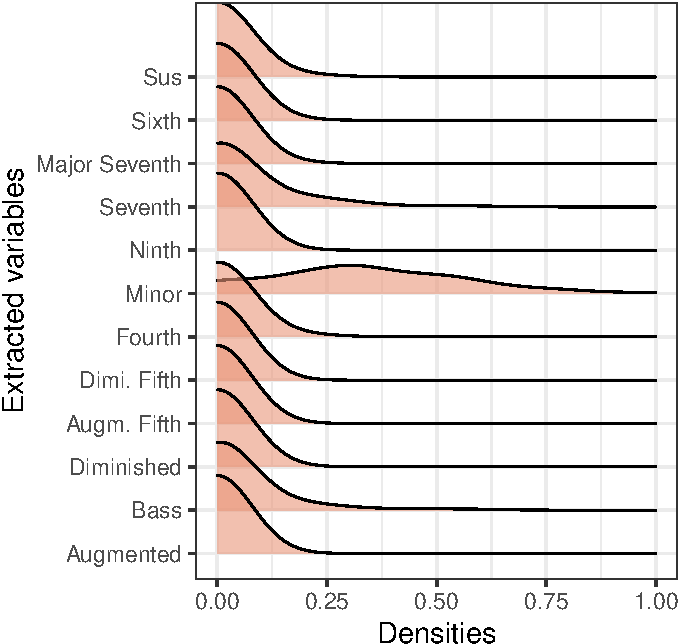
\includegraphics{assign_files/figure-latex/unnamed-chunk-4-1} 

}

\caption{Densities of the extracted features for Muse songs}\label{fig:unnamed-chunk-4}
\end{figure}

The Figure 1 shows us the densities of the features extracted. We can
see that there are not many differences for most of the features. The
only one that stands out a little is the proportion of minor chords in
Muse songs, indicating that they use it a lot when composing.

\begin{Shaded}
\begin{Highlighting}[]
\KeywordTok{source}\NormalTok{(}\StringTok{"assignment/credentials.R"}\NormalTok{)}

\CommentTok{# obtaining lyrics from Muse songs with the Vagalume API}
\NormalTok{lyrics <-}\StringTok{ }\KeywordTok{read.table}\NormalTok{(}\StringTok{"assignment/lyrics.txt"}\NormalTok{)}

\KeywordTok{dim}\NormalTok{(lyrics) }\CommentTok{# 143 rows and 8 columns}

\CommentTok{# applying c function to each lyric}
\NormalTok{fs <-}\StringTok{ }\KeywordTok{list.files}\NormalTok{(}\StringTok{"assignment/lyrics/"}\NormalTok{)}

\NormalTok{res <-}\StringTok{ }\NormalTok{fs }\OperatorTok\StringTok{ }\KeywordTok{map_chr}\NormalTok{(}\OperatorTok{~}\NormalTok{\{}
  \KeywordTok{paste}\NormalTok{(}\KeywordTok{getwd}\NormalTok{(),}\StringTok{"/count "}\NormalTok{, }\KeywordTok{paste0}\NormalTok{(}\StringTok{"assignment/lyrics/"}\NormalTok{, .x) ,}\DataTypeTok{sep=}\StringTok{""}\NormalTok{)\}) }\OperatorTok\StringTok{ }
\StringTok{  }\NormalTok{purrr}\OperatorTok{::}\KeywordTok{map_chr}\NormalTok{(}\OperatorTok{~}\NormalTok{\{}\KeywordTok{system}\NormalTok{(.x, }\DataTypeTok{intern =} \OtherTok{TRUE}\NormalTok{)\})}

\CommentTok{# obtaining formatted results }
\NormalTok{df <-}\StringTok{ }\KeywordTok{data.frame}\NormalTok{(}
  \DataTypeTok{song =}\NormalTok{ lyrics}\OperatorTok{$}\NormalTok{song,}
  \DataTypeTok{n_words =} \KeywordTok{str_extract}\NormalTok{(res, }\StringTok{"[0-9]\{1,5\}"}\NormalTok{) }\OperatorTok\StringTok{ }\KeywordTok{as.numeric}\NormalTok{())}
\end{Highlighting}
\end{Shaded}

\begin{Shaded}
\begin{Highlighting}[]
\CommentTok{# visualizing it!}
\NormalTok{df }\OperatorTok\StringTok{ }
\StringTok{  }\KeywordTok{ggplot}\NormalTok{(}\KeywordTok{aes}\NormalTok{(}\KeywordTok{reorder}\NormalTok{(song, n_words), n_words)) }\OperatorTok{+}
\StringTok{  }\KeywordTok{geom_bar}\NormalTok{(}\DataTypeTok{alpha =} \FloatTok{0.6}\NormalTok{, }\DataTypeTok{stat =} \StringTok{"identity"}\NormalTok{, }\DataTypeTok{fill =} \StringTok{"darksalmon"}\NormalTok{) }\OperatorTok{+}
\StringTok{  }\KeywordTok{guides}\NormalTok{(}\DataTypeTok{fill =} \OtherTok{FALSE}\NormalTok{) }\OperatorTok{+}
\StringTok{  }\KeywordTok{coord_flip}\NormalTok{() }\OperatorTok{+}
\StringTok{  }\KeywordTok{labs}\NormalTok{(}\DataTypeTok{x =} \StringTok{"Songs"}\NormalTok{, }\DataTypeTok{y =} \StringTok{"Number of words"}\NormalTok{) }\OperatorTok{+}
\StringTok{  }\KeywordTok{theme_bw}\NormalTok{(}\DecValTok{10}\NormalTok{)}
\end{Highlighting}
\end{Shaded}

\begin{figure}[H]

{\centering 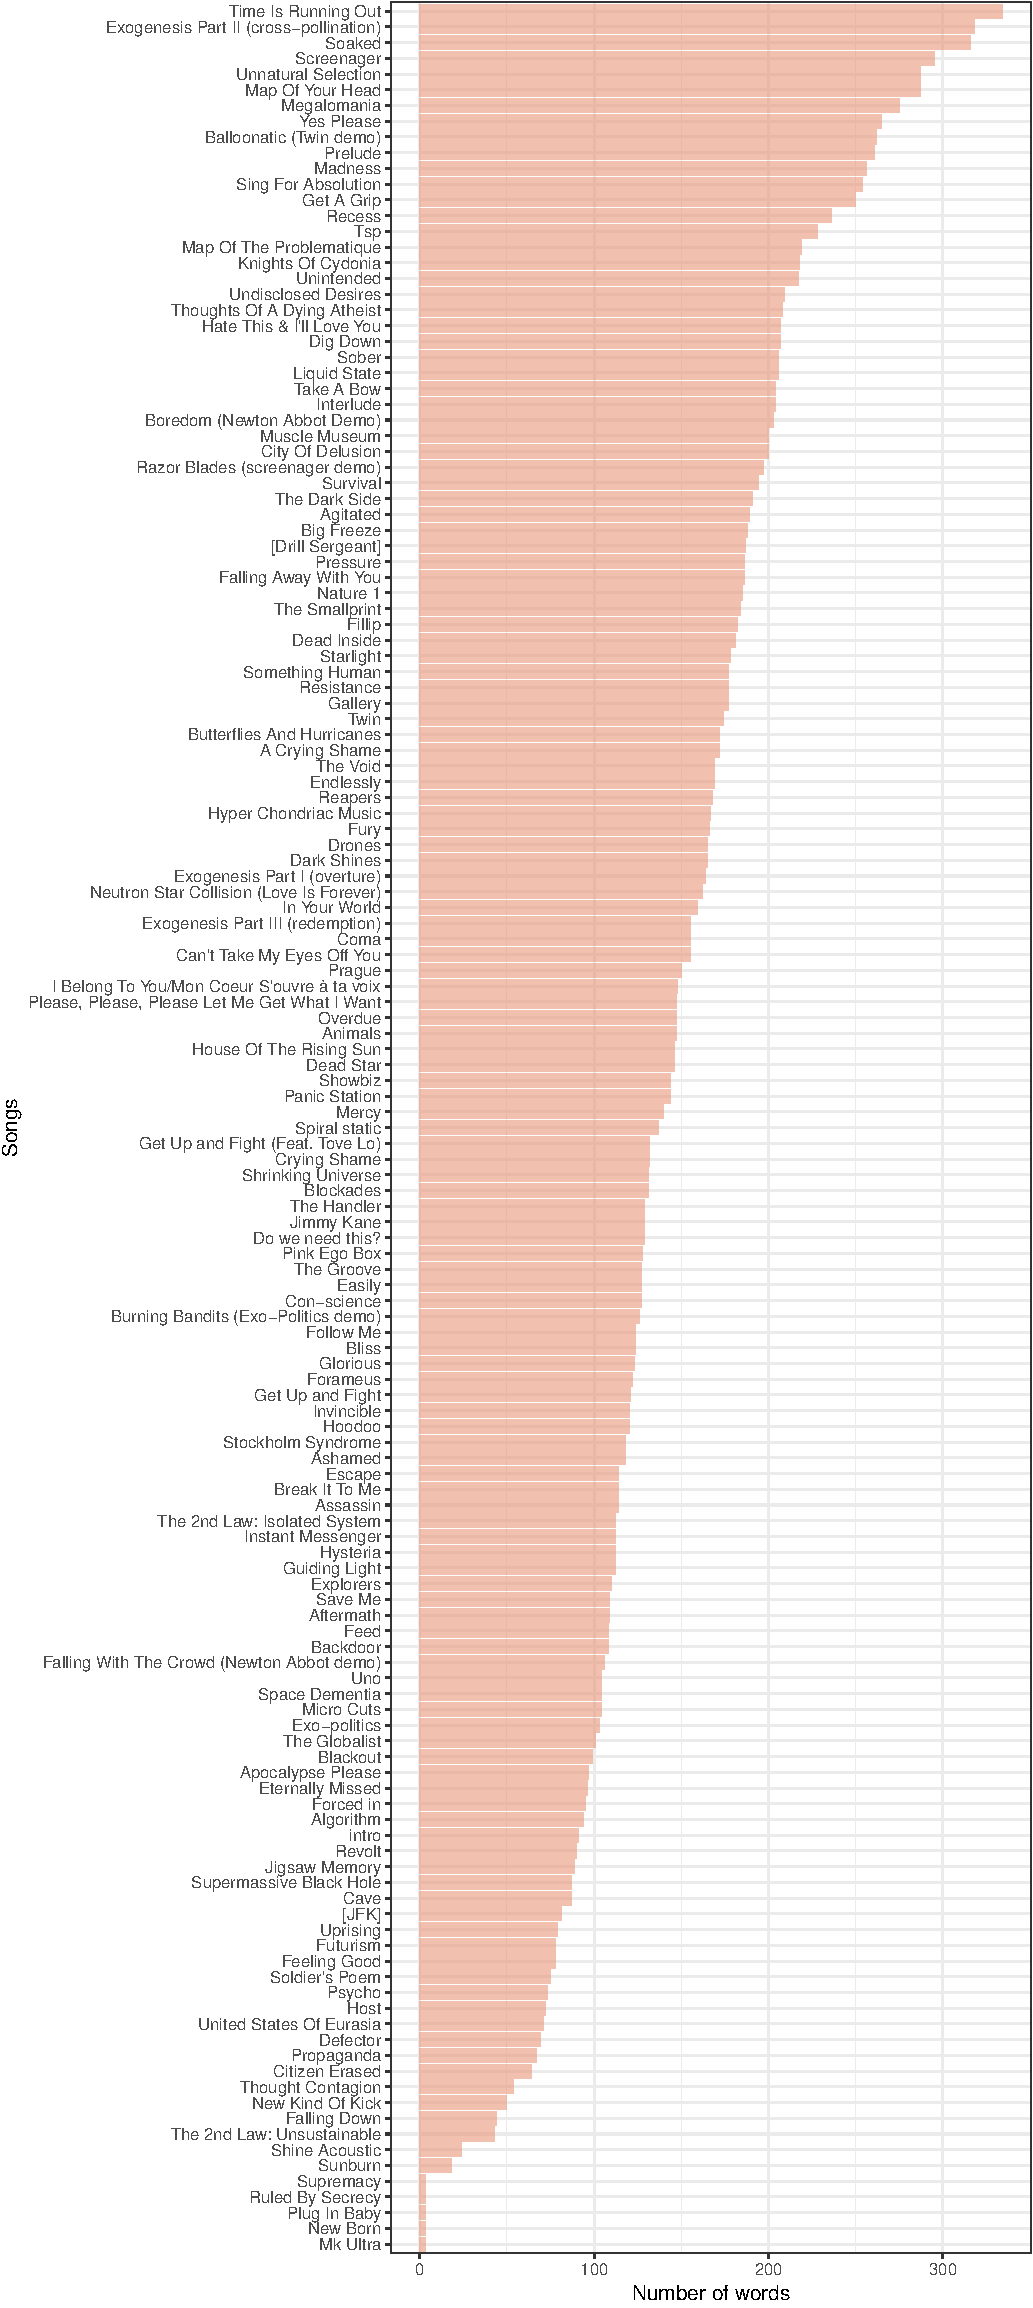
\includegraphics{assign_files/figure-latex/unnamed-chunk-7-1} 

}

\caption{Word counts for each Muse song found in the Vagalume website}\label{fig:unnamed-chunk-7}
\end{figure}

Figure 2, on the other hand, shows us the word counts for each song. We
can see that some songs do not have many words, which probably means
that they are mostly instrumental. Other songs have many words, showing
that they are more focused on the lyrics, since that is a strong
characteristic of the Muse band.

\bibliography{bibliography.bib}


\end{document}
